\documentclass[10pt]{article}
\usepackage[utf8]{inputenc}
\usepackage{parskip}
\usepackage[a4paper, margin=1.5in]{geometry}
\usepackage{graphicx}
\usepackage{hyperref}
\usepackage{listings}
\usepackage{array}

\renewcommand{\arraystretch}{1.5}

\title{Task 1 Report}
\date{11/11/2019}
\author{Federico Fregosi, Mirko Laruina,\\
        Riccardo Mancini, Gianmarco Petrelli}

\begin{document}
\pagenumbering{gobble}
\maketitle
\vfill
% \setcounter{tocdepth}{1}
\tableofcontents
\vfill
\clearpage
\setcounter{page}{1}
\pagenumbering{arabic}

\section{Application Specifications}
\subsection{Application overview}
The application is a messaging system where registered users can create an 
account, exchange text messages and make groups.

A registered user can initiate a chat with another user, create a new group chat
(of which he becomes the admin) and send messages to the chats he belongs to,
as well as receiving messages from those chats. He can also leave a group.

A group admin can add and remove new users to the group. He cannot assign his
powers to another user in the group and if he leaves the group, the latter 
is deleted.

Everytime a user views a chat, all the latest messages from the chat are fetched from 
the server and shown to the user.

\subsection{Actors}
Anonymous user, registered user, group admin and a time-based event.

\subsection{Requirement Analysis}
\subsubsection{Functional requirements}

An \textbf{anonymous user} must be able to register in order to become a 
\emph{registered user}. Registration is done by providing a username and a 
password. Once registered, the user can login using the provided credentials. 
Every user must have a different username.

Log-out of a user is performed through a dedicated button. If the user closes 
the application without logging-out, he will not need to perform another login 
when reopening the application within 5 days.

A \textbf{registered user} must be able to:
\begin{itemize}
    \item Retrieve the list of chats she's a member of
    \item Read the messages of a chat
    \item Send a message to a chat
    \item Create a new private chat
    \item Create a new group chat
    \item Leave a group chat
\end{itemize}

In order to create a private or group chat, the user must type in the username
of the other participants.
When an user create a new group chat, he automatically becomes the admin of the chat in question.

A \textbf{group admin} is the only chat member who is be able to:
\begin{itemize}
    \item Add members to the group chat
    \item Remove users from the group chat
    \item Delete the group chat
\end{itemize}

Adding an user to the group requires once again to specify the username of the 
correspondent. 

The administrator of a chat cannot leave the chat (he can only delete it).

The \textbf{time-based event} updates the user interface on regular intervals
to show chat updates, i.e. new chats or new messages from the current chat, if any.

\subsubsection{Non-Functional requirements}
\begin{itemize}
	\item \textbf{Data concurrency:} the application must be able to handle concurrent requests to the database remaining consistent between every operation even with high volume of data. 
	
	\item \textbf{Real-time updates:} A (soft) real-time updating component that pulls updates from the server is also required for this type of application in order to to ensure a comfortable and efficient use.
	
	\item \textbf{Responsiveness and cross-platform:} Client-side application must provide a responsive view both for pc, laptops and mobile devices.
	
	% \item \textbf{Scalability:} At the increase of the storage occupancy of a chat (single or group one) the access and download time of the chat must remain almost constant. This is possible by implementing a partial and/or "on request" loading rather than from scratch.
\end{itemize}

\clearpage
\section{Design}
\subsection{Use-case diagram}
\begin{figure}[h!]
    \centering
    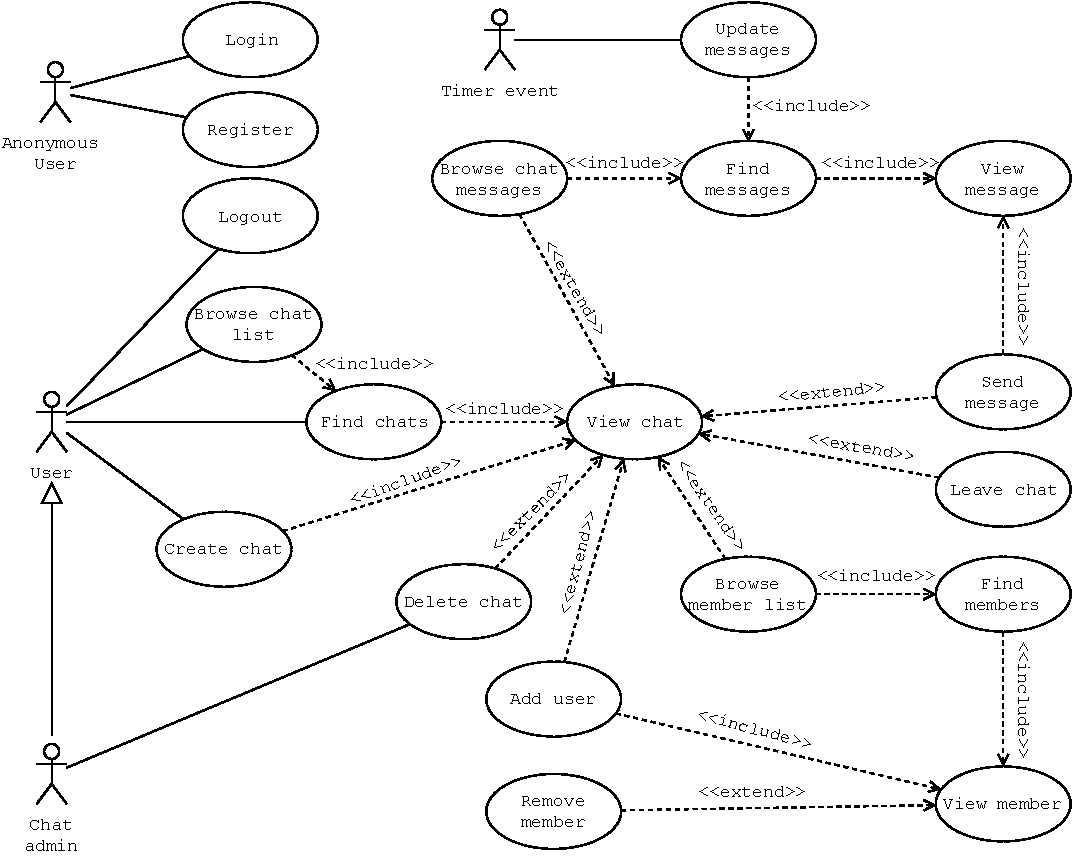
\includegraphics[width=\textwidth]{figs/use_case_diagram}
    \caption{Use-case diagram. Use-cases indicated with a star (\texttt{*})
        require the user to be the chat administrator.}
    \label{fig:usecase}
\end{figure}

\subsection{Class diagram}
\begin{figure}[h!]
    \centering
    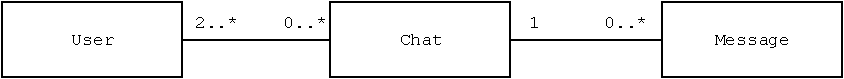
\includegraphics[width=\textwidth]{figs/class_diagram}
    \caption{Class diagram for the identified entities}
    \label{fig:class_diagram}
\end{figure}

It can be seen that we chose to keep it as simple as possible by not making  
any distinction between \emph{private chats} and \emph{group chats}, 
creating a single \emph{Chat} entity.
\clearpage
\subsection{Software Architecture}
\begin{figure}[h!]
	\centering
	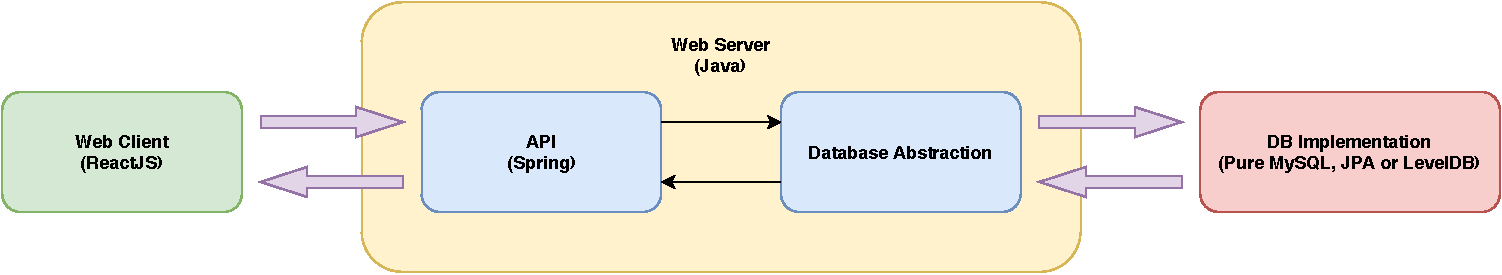
\includegraphics[width=\textwidth]{figs/system_architecture}
	\caption{EasyChat software architecture}
	\label{fig:software_architecture}
\end{figure}

As can be seen, a Java server back-end is the core of the proposed architecture, providing both the APIs, through the open source Spring Framework, and the database interface, which has to allow a high flexibility in terms of database implementation.

Client-side, a ReactJS front-end has been chosen for the implementation of the web app the user will interact with.


\clearpage
\section{Implementation}

\subsection{Database}
\subsubsection{Relational DB Design}
\begin{figure}[h!]
    \centering
    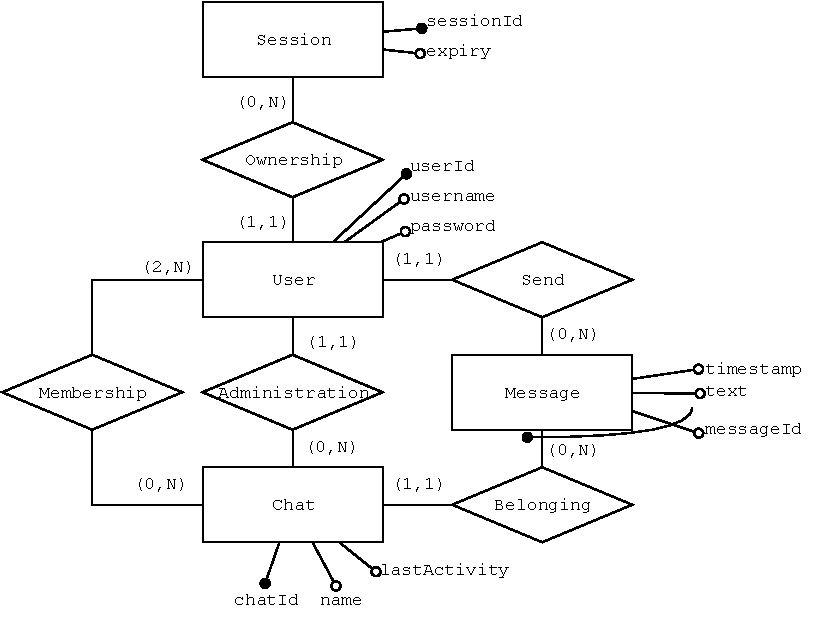
\includegraphics[width=\textwidth]{figs/ER}
    \caption{ER diagram for the database.}
    \label{fig:er}
\end{figure}

Figure~\ref{fig:er} shows the ER diagram of the MySQL database. Every \emph{User} 
is identified a \emph{userId} and has got a unique \emph{username} and a 
\emph{password}. The user can be a member of many \emph{Chats} and can 
be the administrator of many \emph{Chats}. On the other hand, a \emph{Chat} 
can be administered by only one \emph{User}. A \emph{User} can send a 
\emph{Message} to a \emph{Chat}. Each \emph{User} and each \emph{Chat} can 
have many \emph{Messages} while a \emph{Message} can belong to one \emph{Chat}
and one \emph{User} only. The \emph{Session} represents a logged user session.
Each \emph{User} can have many open \emph{Sessions}.

Once the database had been created, we filled it with random test data using the free
service available at \url{http://filldb.info/}. Generated data is not perfect, 
since some more complex functional constraints could not be included in the 
generation. However, that was sufficient for the first functional tests of the
application.

\subsection{Java backend}
The Java backend provides simple REST APIs for managing the chat application. 
In order to do so, it uses the \emph{Spring} framework\footnote{More information
at \url{https://spring.io/}}.
The list of the APIs and their description can be found in the 
\texttt{docs/api.md} file. The APIs return a JSON document, generated using
\emph{Google GSON}\footnote{More information at 
\url{https://github.com/google/gson}}, which is interpreted and shown to the user
by the ReactJS frontend.
These APIs are implemented using a simple database abstraction layer which provides 
corresponding APIs to the database. This is implemented in Java 
using a generic \emph{DatabaseAdapter} interface that can be implemented to 
provide access to different databases (as we have done in this Task with plain SQL, 
JPA and levelDB implementations). The database backend can be set from a configuration
file, where some other db-specific settings can be set.

\subsubsection{JPA}
Once the database design was set, the Java implementation of the methods using 
JPA was very easy and fast. A new implementation of the \emph{DatabaseAdapter}
class has been done, along with JPA implementations of the data model interfaces.
Both one-to-many and many-to-many relationships have been used. A more detailed 
explanation of the JPA implementation can be found in the tutorial.

\subsection{ReactJS frontend}
The frontend has been developed using the \emph{ReactJS} framework\footnote{More
information at \url{https://reactjs.org/}}. An overview of the main functions 
is available in the user guide (\texttt{docs/user\_guide/user\_guide.pdf}).

Regarding the implementation, the most notable thing is the timer-based event
that updates the UI. In particular, the client makes a request to the server
every second for updating the list of chats and every half second for updating 
the list of messages in the current chat.

\subsection{Limitations}
\paragraph{Passwords}
For the sake of simplicity, password hashing has not been implemented into the 
application. However, this could be simply integrated with a future update.

\paragraph{Polling}
In the current implementation, the server is polled every second for updating 
the list of chats and every half second for updating the list of messages. This 
is indeed a great load on the server in case there are many clients connected 
at the same moment. 
This problem has been alleviated by requesting only a subset of the chat 
messages, based on the timestamp on the latest received message.
However, 
a more appropriate way to handle it would be having a kind of notification API
that can be ``long polled''\footnote{A ``long poll'' is when the client 
makes a request to the server and the server does not respond until new 
information is available, at the cost of timing out the connection, at which 
point a new request is made.} by the client.

\clearpage
\section{Testing and Evaluation}
The application has been tested using unit tests and a final integration test.

\subsection{Unit tests}
The database APIs have been tested using unit tests through \emph{JUnit4}
\footnote{More information at \url{https://junit.org/junit4/}} before being 
integrated with the API backend code. In particular, every method in 
\emph{DatabaseAdapter} is tested against sample data, verifying its result.

These automated unit tests made it possible to identify bugs at their root cause,
saving a lot of time in debugging.

\subsection{Integration test}
In the end, once everything had been put together, we performed a final test 
in order to verify the correctness of all use cases.

\end{document}
